\documentclass{article}
\usepackage[T1]{fontenc}
\usepackage{lmodern}
\usepackage{graphicx}
\usepackage{amsmath,amssymb}
\usepackage[a4paper,margin=2cm]{geometry}
\usepackage[absolute,overlay]{textpos}
\setlength{\TPHorizModule}{1mm}
\setlength{\TPVertModule}{1mm}
\usepackage[indonesian]{babel}
\usepackage{hyperref}
\setlength{\emergencystretch}{2em}
% unit: Halaman 52

\begin{document}

% === Halaman 52 (llm) ===

\section*{Triple DES}

\vspace{71.28mm}

\textbf{Triple DES dengan 2 kunci (56 + 56 = 112 bit)}

\vspace{20mm}

\vspace{20mm}

% deskripsi: Diagram proses enkripsi Triple DES dengan 2 kunci (K1, K2, K1) yang terdiri dari tahap enkripsi (E), dekripsi (D), dan enkripsi (E) kembali.
% bbox normalisasi: [0.1800, 0.3400, 0.6700, 0.5800]
\begin{textblock*}{102.90mm}(37.80mm,100.98mm)
\noindent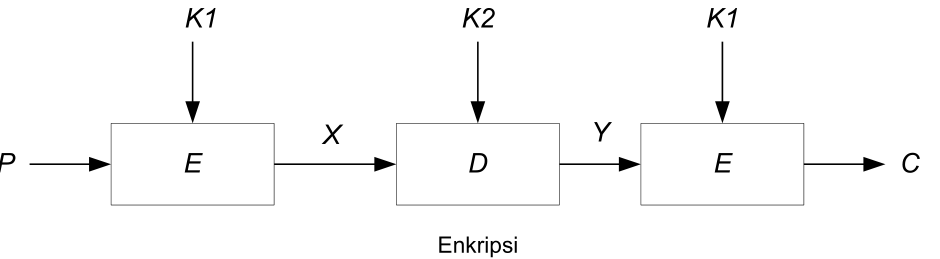
\includegraphics[width=102.90mm,height=71.28mm]{../../images/llm/page_052_img_01.png}%
\end{textblock*}

% deskripsi: Diagram proses dekripsi Triple DES dengan 2 kunci yang merupakan kebalikan dari proses enkripsi, terdiri dari tahap dekripsi (D), enkripsi (E), dan dekripsi (D) kembali.
% bbox normalisasi: [0.1800, 0.6200, 0.6700, 0.8700]
\begin{textblock*}{102.90mm}(37.80mm,184.14mm)
\noindent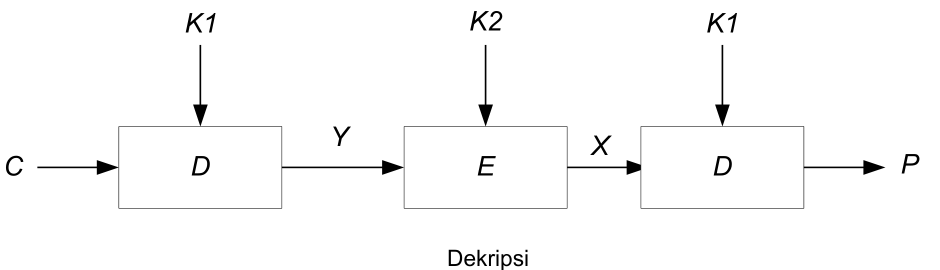
\includegraphics[width=102.90mm,height=74.25mm]{../../images/llm/page_052_img_02.png}%
\end{textblock*}

\end{document}
